\documentclass[a4paper,11pt]{article}
\usepackage{amsmath}
\usepackage{graphicx}
\usepackage{hyperref}
\usepackage{float}
\usepackage{geometry}


\usepackage{listings} % Pour afficher le code
\usepackage{xcolor}   % Pour les couleurs du code

\definecolor{codegreen}{rgb}{0,0.6,0}
\definecolor{codegray}{rgb}{0.5,0.5,0.5}
\definecolor{codepurple}{rgb}{0.58,0,0.82}
\definecolor{backcolour}{rgb}{0.95,0.95,0.92}

\lstset{
    language=Python,
    backgroundcolor=\color{backcolour},   % Couleur d'arrière-plan
    commentstyle=\color{codegreen},       % Style des commentaires
    keywordstyle=\color{magenta},         % Style des mots-clés
    stringstyle=\color{codepurple},       % Style des chaînes
    basicstyle=\ttfamily\footnotesize,    % Style de base
    numberstyle=\tiny\color{codegray},    % Style des numéros de ligne
    numbers=left,                         % Numéros de ligne
    numbersep=5pt,                        % Espace entre les numéros et le code
    frame=single,                         % Ajoute un cadre
    showstringspaces=false,               % Désactive l'affichage des espaces
    tabsize=4,                            % Largeur d'une tabulation
    breaklines=true,                      % Casse les lignes longues
    captionpos=b,                         % Position de la légende
}
\geometry{margin=1in}

\title{Automatic Detection of Hyperparameters in Datasets \\
       \large Predictions for Nearest Neighbor Models}
\author{Alexis Rosenfeld \& François Delafontaine}
\date{Fall 2024}

\begin{document}

\maketitle

\begin{abstract}
    This report investigates meta-learning techniques for predicting the optimal \(k\) in \(k\)-Nearest Neighbors (KNN) models. It does so by generating synthetic datasets, extracting meta-features from them and testing linear regression and neural network models. The presentation of each step is followed by a discussion on performance metrics and will emphasize the effects our dataset generation had on the results.
    \newline
    \newline
    The source code for this project is available at :
\newline
\href{https://github.com/AlexisRosenfeld/Project_IntroML_2024/}{\small\textcolor{blue}{https://github.com/AlexisRosenfeld/Project\_IntroML\_2024/}}.
\end{abstract}

\tableofcontents

\section{Meta-learning}
\begin{quote}
    Meta-learning, or \emph{learning to learn}, is the science of systematically observing how different machine learning approaches perform on a wide range of learning tasks, and then learning from this experience, or meta-data, to learn new tasks much faster than otherwise possible.
\begin{flushright}
— Hutter, F., Kotthoff, L., \& Vanschoren, J. (2019). \emph{Automated Machine Learning: Methods, Systems, Challenges} (p. 219). Springer Nature.
\end{flushright}
\end{quote}

\textit{Meta-learning} refers here to training a model on a task that is itself part of training a model, in this case the selection of hyperparameters. To further limit the scope of the task, it is limited to the \(k\)-Nearest Neighbors (KNN) model for its single \(k\) hyperparameter, and further constrained to purely quantitative datasets from which the hyperparameter should be derived.

We therefore have datasets with features and an optimal \(k\) hyperparameter; we can derive \textit{meta-features} from those datasets, such as dataset size, dimensionality, statistical moments, etc. and then train a model on those \textit{meta-features} to predict the best \(k\) value.

The primary objective is to reduce the computational cost of finding \(k\) from \(O(n^2)\) to \(O(1)\) using a predictive model instead of computationally expensive methods such as grid search or cross-validation. 

All the source code used in this report can be found in the \textit{kguesser.py} file.

\section{Data and features}
The project planned for three sources of datasets:
\begin{enumerate}
    \item \textit{Test datasets}: Generated by defining the meta-features first and then calculating a \(k\) through KNN iterations; the purpose being to observe the relations between meta-features and \(k\).
    \item \textit{Simulated datasets}: Generated by setting \(k\) first, followed by the calculation of meta-features through pre-defined relations; the purpose being to test the model's behavior in a fully-controlled environment.
    \item \textit{Real datasets}: Sourced from publicly available repositories; the purpose being to evaluate the model's actual performance. 
\end{enumerate}
In practice, only Test datasets have been exploited, as it has proved difficult to determine relationships for the selected meta-features. 

As for those meta-features, they were selected based on a few assumptions as to those relations. One was that \(k = \sqrt{n}/2\), as an approximation where \(n\) is the number of samples in the dataset. Another assumption was that the more noise, understood here as the overlap of feature values, the higher the \(k\) value should be. Yet another assumption was that the type of distribution could affect \(k\), although the types and manner were unclear. 

As a result, we selected the following:
\begin{itemize}
    \item \(n\_rows\): Number of samples.
    \item \(n\_classes\): Number of unique labels in the target variable.
    \item \(n\_features\): Number of predictors.
    \item \(n\_nonrand\): Count of non-random features (weighed by correlation).
    \item \(distr\_type\): Distribution type (linear, quadratic, etc.).
    \item \(distr\_noise\): Overlap likelihood of feature values.
    \item \(mean\_var\): Weighted mean of feature variances.
    \item \(mean\_skew\): Weighted mean of feature skewness.
    \item \(mean\_kurtosis\): Weighted mean of feature kurtosis.
\end{itemize}

Three types of distribution were implemented: a linear relation to \(k\), a quadratic one and a probabilistic relation with \(20\%\) random datapoints. As for the noise, it is a categorical meta-feature with three values based on the overlap likelihood of a feature's values relative to \(k\). 

\begin{figure}[ht]
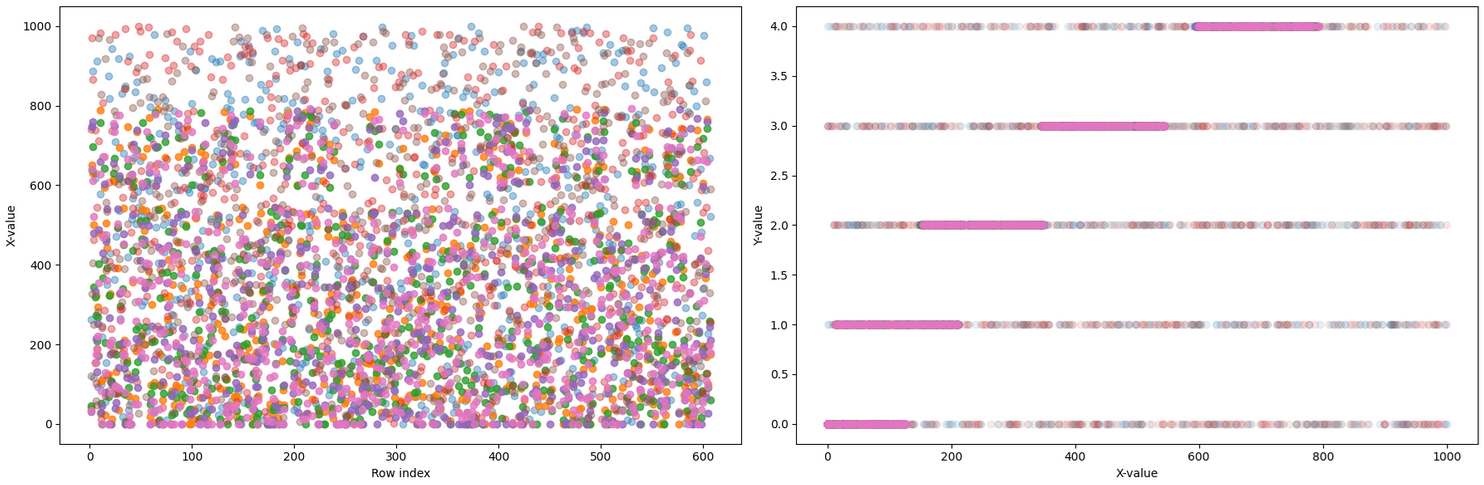
\includegraphics[width=\textwidth]{Img/dataset.png}
\caption{Illustration of a dataset.}
\end{figure}

Figure 1 showcases a generated dataset with 7 features and 600 datapoints. Each feature has a quantitative value in the \([0-1000]\) interval. The second graph shows a quadratic distribution with little noise, visible especially on the higher \(y\) values where no overlap occurs.

\begin{figure}[ht]
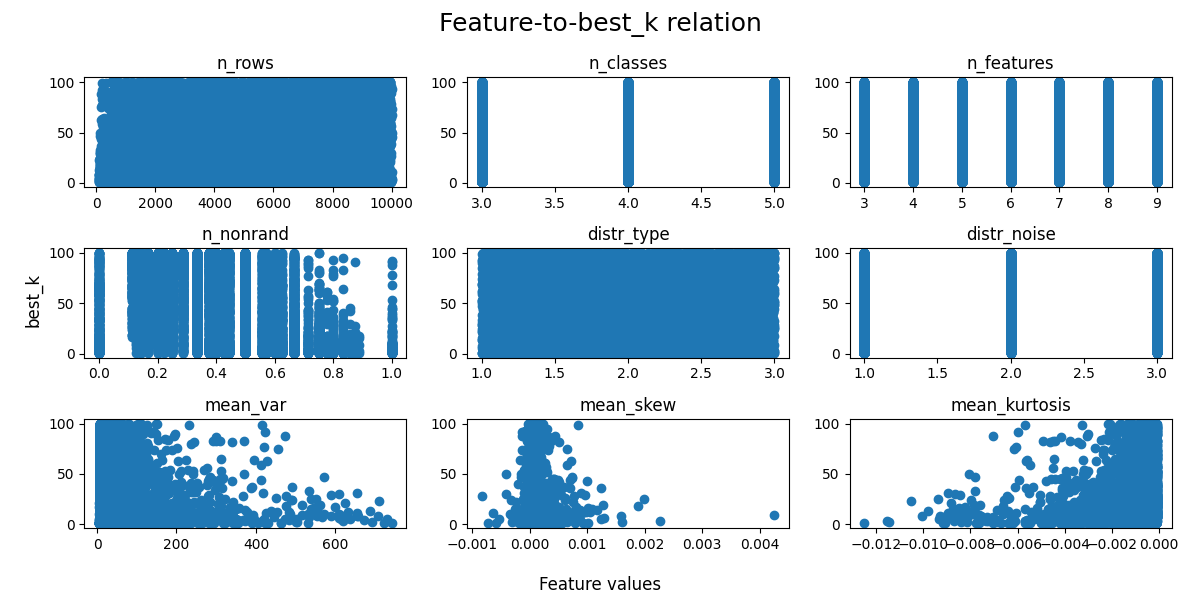
\includegraphics[width=\textwidth]{Img/relations.png}
\caption{Meta-feature relations.}
\end{figure}

Figure 2 presents the observed relations between our meta-features and the \(k\) hyperparameter based on 10,000 datapoints. We cannot discern clear relations from this, especially where expected with the number of rows; and while the statistical moments seem to follow a distribution, it is hard to interpret, especially as those moments are bound to be interdependent. 

This speaks to not just the complexity of the task, with Real datasets expected to be even noisier, but also of our Test datasets. By testing three assumptions at once, the results became unreadable, preventing the establishment of relations for proper simulation work.

All operations to generate datasets is handled by the \textit{KG\_test} class.

\section{Models and pipeline}

The \(k\) hyperparameter is a quantitative value. We therefore focused on regression models, the simplest of which being the linear regression. The results eventually pushed us to test a more complex model; for that role we chose a neural network (NN). The pipeline in both cases is the same. The data is 10,000 datapoints containing our meta-features and the optimal \(k\) value.

We will already provide the evaluation of each model in this section but discuss those results in a later section. The evaluation was done by splitting our data into training and evaluation, then doing a 5-folds cross-evaluation on the training data, then fitting the training data, predicting with the evaluation data and measuring the \textit{Mean Squared Error} (MSE) and \textit{Coefficient of Determination} (\(R^2\)). Results will focus mainly on the latter.

All operations regarding the pipeline is handled by the \textit{KG\_model} class.

\subsection{Preprocessing}
Before training and evaluating the model(s), three steps were necessary:
\begin{enumerate}
    \item \textbf{One-Hot Encoding:} Transforming categorical features.
    \item \textbf{Scaling:} Standardizing feature values for numerical stability.
    \item \textbf{Feature Selection:} Retaining features by correlation.
\end{enumerate}
Regarding the selection of meta-features, it eliminates by default any meta-feature with a correlation score \(<= 0.2\). For our data, only \textit{n\_nonrand} and \textit{distr\_noise} cleared that threshold and were kept. 

More precisely, feature selection is the last pre-process step, so while we preserved all values of \text{distr\_noise}, it had by then already been encoded and it would be more accurate to say that \textit{distr\_noise\_1} alone, that is the lowest noise level, cleared that threshold. This suggests that a better categorization of noise is required; but because that value may prove impossible to extract from Real data and because a correlation above 0.2 can still prove insufficient, it is likely not worth pursuing.

\subsection{Regression Model}
While meta-features are hard to determine, extract and select, the task itself is relatively simple and the relations expected to be straightforward. Therefore, a \textit{linear regression} model was deemed sufficient.

We expected \textit{n\_rows} to be significant and have a logarithmic relation; we likewise observed an exponential relation for \textit{mean\_var}. Those could have been reduced to linear relations by applying their inverse as a first preprocess step, before scaling. But with \textit{n\_nonrand} and \textit{distr\_noise} being the meta-features, none of those considerations became relevant. Instead, the model became:
\[
k = \beta_0 + \beta_1 n\_nonrand + \beta_2 distr\_noise\_1 + \beta_3 distr\_noise\_2 + \beta_4 distr\_noise\_3
\]
When trained and evaluated, the linear regression model offered:
\begin{itemize}
    \item A cross-validation score (\(R^2\)) of 0.25
    \item An MSE of 809.1
    \item An \(R^2\) of 0.2
\end{itemize}

\subsection{Neural Network}
Given the results obtained through a linear regression, we wanted to test if the model was at fault. We did not expect a \textit{RandomForest} to be adapted to a limited number of quantitative features and therefore resorted to a neural network (NN). 

For an NN model it is necessary to detail the parameters:
\begin{itemize}
    \item Layers: \([x, 64, 64, 32]\)
    \item Activation: Relu
    \item Optimization: lbfgs, sgd, adam
\end{itemize}
We tested a few layer patterns and settled on the current one. It is likely far too big for the task but again, our goal was to test whether bad performances were due to models being too simple. As for optimization, we tested three of them, albeit without touching the learning rate for \textit{sgd} or optimizing the betas for \textit{adam}. 

That is because we obtained:
\begin{itemize}
    \item MSEs around 679-732
    \item \(R^2\) between 0.31-0.36
\end{itemize}
With the \textit{lbfgs} optimizer performing best, at 0.36, giving us little reason to seek and optimize the others.

\section{Performances}
This report would not be complete without discussing the results we observed. The models we built, whether linear regression or neural networks, seek to return an optimal \(k\) value for the user; with an evaluation score of 0.2-0.36, we can accept that this task is not fulfilled.

This brings two questions. 

The first is what to fault for the results. At this stage we would safely rule out the choice of model as, while the neural network performs better, it is still insufficient. So the question then becomes whether the problem lies in our meta-features or with the Test datasets themselves. 

The second question is whether that evaluation metric is the right one. If our model should return a \(k\) value, the user will evaluate it through the KNN performance. This, in turn, will prove to simplify the problem greatly.

\subsection{Performance Metrics}
There are several faults in our meta-features. We have already observed how the distribution noise values may not represent the right steps to properly inform on how noisy the data actually is; and more generally, how that distribution noise might not even be accessible to the user. We can also fault the distribution type: it should be a categorical value but, through its implementation, it turned into a quantitative one. This is a flaw that was left unaddressed simply because, regardless, no relationship appeared anyway.

Meanwhile, that no relationship can be visible for the number of rows is abnormal. What this suggests to us is that the generation of datasets itself is at fault. 

We expect it to be too complex and, as a result, too noisy. It was in fact designed to generate noisy data as prior exploratory work, generating clearer datasets, had the number of rows being the sole, overwhelming meta-feature. Further work on meta-learning for the \(k\) hyperparameter should focus on a single assumption, simulate on simpler datasets and then test on real datasets to avoid the current situation. 

\subsection{Accuracy}
Saying that our dataset generation is at fault becomes even clearer when considering how the predicted \(k\) actually performs on the dataset. That is to say, we can evaluate our models not on how off they are on selecting a \(k\) but on what accuracy the KNN gets from that \(k\) hyperparameter. The evaluation is between the accuracy obtained by the optimal \(k\) and the accuracy from the predicted one. 
\begin{itemize}
    \item 0.99 for the linear regression
    \item 0.98 for the neural network (lbfgs)
\end{itemize}
The reason behind such impressive results is that most datasets allow for +40 \(k\) margin before accuracy falls by more than 0.1. Some datasets, especially for the lower accuracies, don't have any variation at all. In such conditions, any model with any amount of training data (we tested with as few as 80 datapoints) is bound to perform well.

\section{Discussion}
Meta-learning offers great perspectives for the automatic selection of hyperparameters. For the KNN model in particular, we can expect just a few meta-features to suffice: in a good dataset, those meta-features will provide a decent approximation while in a noisy or faulty dataset, any hyperparameter value becomes valid. The model could really be as simple as:
\[
k = \sqrt{n}/2
\]
But statistical moments, and correlation, may prove helpful as well.

As for our methodology, we thought wise to first observe how even synthetic datasets behaved to determine the relations for our meta-features. This report can only conclude that such an approach must be abandoned or, at the very least, should have worked with much simpler and cleaner datasets. 

Simulations are there either to prepare an experiment, that is to see if the methodology will be viable before expending resources on it, or to test an experiment, that is to see how the model perform under controlled data. By not preparing anything and just assuming that our synthetic datasets would be good enough, our entire project had been set to fail from the start.

\appendix

\section{References}
\begin{thebibliography}{9}
\bibitem{hutter2019}
F. Hutter, L. Kotthoff, J. Vanschoren, \textit{Automated Machine Learning: Methods, Systems, Challenges}, Springer, 2019.
\end{thebibliography}

\section{Appendix - Python code} 
%
%
\begin{lstlisting}[caption={Operations}, label={lst:python_code}]
    from kguesser import KG_test, KG_model      # import kguesser classes

        # data generation
    kg_test = KG_test()
    dat, k = kg_test.sim(n, d_path, k_path)     # generate data and k tables
    kg_test.show_features(dat)                  # plot relations
        # pipeline
    kg_model = KG_model()
    dat = kg_model.load(d_path)                 # load data
    kg_model.ktab = None                        # remove k table
    kg_model.load_k(k_path)                     # load k table
    mean, std, mse, r2 = kg_model.test_lm(dat)  # linear regression
    for o in ['lbfgs', 'sgd', 'adam']:          # test NN optimizers
        mean, std, mse, r2 = kg_model.test_nn(dat, params={'solver':o}, 
                                              cross=False)
    mean, std, mse, r2 = kg_model.test_nn(dat)  # neural network
\end{lstlisting}
%

%

%

\end{document}